%%%%%%%%%%%%%%%%%%%%%%%%%%%%%%%%%%%%%%%%%%%%%%%%%%%%%%%%%%%%%%%%%%%%%%%%%%%%%%%%%%%%%%%%%%%%%%%%%%%%%
% This template is distributed with ABSOLUTELY NO WARRANTY.
% It serves as a guideline and constitutes a basic structure for a
% thesis/dissertation. The user assumes full responsibility for formatting
% and typesetting their document and for verifying that all the thesis
% requirements set by the University of Tennessee are met. Please refer to the most
% recent UT thesis guide (http://web.utk.edu/~thesis/thesisresources.shtml)
% or contact the thesis consultant (http://web.utk.edu/~thesis/).
% Please report any bugs to the thesis consultant.
%%%%%%%%%%%%%%%%%%%%%%%%%%%%%%%%%%%%%%%%%%%%%%%%%%%%%%%%%%%%%%%%%%%%%%%%%%%%%%%%%%%%%%%%%%%%%%%%%%%%%
% O P T I O N S:
% 1. thesis/dissertation
% 2. monochrome
% 3. all options provided by the report class
\documentclass[dissertation,letterpaper,12pt]{utthesis} % thesis, one side
% some alternatives are:
%\documentclass[thesis,monochrome,letterpaper,12pt]{utthesis} %thesis, one side, monochrome text
%\documentclass[thesis,twoside,letterpaper,12pt]{utthesis} % thesis, two side
%\documentclass[thesis,monochrome,twoside,letterpaper,12pt]{utthesis} % thesis, two side, monochrome text
% for a dissertation, replace the thesis option by dissertation:
% \documentclass[dissertation,letterpaper,12pt]{utthesis} . . .
\renewcommand{\baselinestretch}{1.5} 	 % line Spacing
%%%%%%%%%%%%%%%%%%%%%%%%%%%%%%%%%%%%%%%%%%%%%%%%%%%%%%%%%%%%%%%%%%%%%%%%%%%%%%%%%%%%%%%%%%%%%%%%%%%%%
% TO DO: FILL IN YOUR INFORMATION BELOW - READ THIS SECTION CAREFULLY
%%%%%%%%%%%%%%%%%%%%%%%%%%%%%%%%%%%%%%%%%%%%%%%%%%%%%%%%%%%%%%%%%%%%%%%%%%%%%%%%%%%%%%%%%%%%%%%%%%%%%
\title{Production of electrons from heavy flavor decays in proton-lead collisions measured with ALICE at the LHC}	       % title of thesis/dissertation
\author{Rebecca Michelle Scott}               % author's name
\copyrightYear{2017}            % copyright year of your thesis/dissertation
\graduationMonth{May}           % month of graduation of your thesis/dissertation
\majorProfessor{Soren Sorensen}	    % advisor's name
\keywords{List, Of, Keywords}	% keywords (optional) separated by commas - these are used in the PDF file properties
\viceProvost{Carolyn R. Hodges} % vice provost name
\major{Physics}	% major: Mechanical Engineering, Aerospace Engineering, Mathematics...
\degree{Doctor of Philosophy}	    % degree: Doctor of Philosophy, Master of Science, Master of Engineering...
\college{Arts and Sciences}           % college
\dept{Physics and Astronomy}	% department
\university{The University  of Tennessee, Knoxville}	% school name
% THIS TEMPLATE ACCOMMODATES UP TO 5 COMMITTEE MEMBERS - ENTER ONLY THE NAMES OF THE MEMBERS ON YOUR COMMITTEE
\numberOfCommitteeMembers{2} % enter the number of committee members
\committeeMemberA {Kenneth Read}	% name of first committee member
\committeeMemberB {Dr. Greene}	% name of second committee member
\committeeMemberC {Dr. Moersch}	% ... you get the trend!
\committeeMemberD {Committee Member 4}	% if your committee has less than 4 members, you do not need to edit the
\committeeMemberE {Committee Member 5}  % rest of committee names
%%%%%%%%%%%%%%%%%%%%%%%%%%%%%%%%%%%%%%%%%%%%%%%%%%%%%%%%%%%%%%%%%%%%%%%%%%%%%%%%%%%%%%%%%%%%%%%%%%%%%
% LOAD SOME USEFUL PACKAGES
%%%%%%%%%%%%%%%%%%%%%%%%%%%%%%%%%%%%%%%%%%%%%%%%%%%%%%%%%%%%%%%%%%%%%%%%%%%%%%%%%%%%%%%%%%%%%%%%%%%%%
\usepackage{nomencl}                    % produces a nomenclature
\usepackage{float}                      % figure floats
\usepackage{natbib}                     % this package allows you to link your references
\usepackage{graphicx}					% graphics package
\graphicspath{ {figures/}{figures/eps/}{figures/pdf/}{figures/pdf/Trigger/}{figures/pdf/Photonic/}{figures/pdf/Alice/}{figures/pdf/EMCal/}{figures/pdf/TPC/}{figures/pdf/ITS/}{figures/pdf/VZERO/}{figures/StandardModel/}{figures/HeavyFlavor/}{figures/chapter1/}{figures/ExperimentalStatus/}{figures/Efficiency/}{figures/FinalResults/}{figures/FONLL/}{figures/centrality/}{figures/EventTrackCuts/}{figures/ITS/}{figures/VZERO/}{figures/ET_and_Nch/}{figures/showershape/}{figures/Fitting/}{figures/systematics/}{figures/chapter5/}{figures/Photonic/}{figures/TriggerScaling/}}% specify the path where figures are located
\usepackage{fancyhdr}                   % fancy headers and footers
\usepackage{url}                        % nicely format url breaks
\usepackage[inactive]{srcltx}		 	% necessary to use forward and inverse searching in DVI
\usepackage{relsize}                    % font sizing hierarchy
\usepackage{booktabs}                   % professional looking tables
\usepackage[config, labelfont={bf}]{caption,subfig} % nice sub figures
\usepackage{mathrsfs}                   % additional math scripts
\usepackage{wrapfig}
%%% PACKAGES THAT ARE PRELOADED WITH THE CLASS ARE: amsmath,amsthm,amssymb,setspace,geometry,hyperref,and color
%%%%%%%%%%%%%%%%%%%%%%%%%%%%%%%%%%%%%%%%%%%%%%%%%%%%%%%%%%%%%%%%%%%%%%%%%%%%%%%%%%%%%%%%%%%%%%%%%%%%%
\begin{document}
    \pagenumbering{alph} % this is needed to clear certain issues with the hyperref package
    %
    %\makeApprovalPage % make the approval page - this is the page that needs to be signed & returned to the thesis/dissertation consultant
    %\makeETDApprovalPage % make the Electronic Thesis & Dissertation page - this page is kept with the electronic copy
    %
    \addToPDFBookmarks{0}{Front Matter}{rootNode} % create a root node named "Front Matter" in the pdf bookmarks
    \addToPDFBookmarks{1}{Title}{a} % add a pdf bookmark to the title page
    \makeTitlePage % make the title page. Make sure you properly set the \docType
    %
    \pagenumbering{roman}
    \setcounter{page}{2}
    %
    \makeCopyrightPage % make the copyright page
    %
%    \addToPDFBookmarks{1}{Dedication}{b} % add a pdf bookmark to the dedication page
%    \chapter*{Dedication}\label{ch:dedication}
सर्वतीर्थमयी माता सर्वदेवमयः पिता 

मातरं पितरं तस्मात् सर्वयत्नेन पूजयेत्
 % include the dedication
    %
    \addToPDFBookmarks{1}{Acknowledgements}{c} % add a pdf bookmark to the acknowledgements page
    \chapter*{Acknowledgements}

I would like to first thank my advisors, Soren Sorensen, Ken Read, and Christine Nattrass for their time, patience and encouragement. I am so thankful that I had the opportunity to learn from three wonderful advisors that each helped me in a unique way.

Having Dr. Nattrass as a role model and mentor was invaluable. She helped me figure out the tiny details that no one else seemed to have the patience for. 

Dr. Read helped me see the super modules for the towers. I could always rely on him to give me honest feedback and help me figure out the best action to take next.

Dr. Sorensen was simply the best advisor I could ever ask for. I will always have a profound debt of gratitude for his scientific guidance and selfless support and encouragement.

I am so grateful that I had the wonderful opportunity to go to CERN and work among the brilliant physicists that make up the ALICE collaboration. I could not have done this without the hard work from my collaborators, and all the engineers and technicians who contributed to the construction, performance and support of the LHC, the ALICE experiment and the Grid. 

In particular I would like to thank Cristiane Jahnke, Shingo Sakai, and Deepa Thomas who taught and helped me so much.

From the UT and ORNL group, I would like to thank Abhisek Sen, David Silvermyr, Matt Wysocki, Natasha Sharma, and Andrew Castro who helped me at different stages of my analysis.

Thanks to Dr. Marianne Breinig and Chrisanne Romeo who were always willing to help and give advice.

I also would like to thank Kyle Schmoll. When I wanted to quit he gave me the encouragement that I needed to continue on. 

I would like to thank my parents, Dora and Antonino Carnevali, who invested in my education and helped me learn to think like a scientist. I would also like to thank my oldest sibling and best friend Alana, and my favorite and only brother Corey.

Lastly, I would like to thank Neutrino, Cappy and Barlow who gave me unconditional love and companionship throughout my time in graduate school.  % include the acknowledgements
    %
    \addToPDFBookmarks{1}{Quote}{d} % add a pdf bookmark to the quotation page
    \chapter*{}
%{\it{If I have seen further, it is by standing on the shoulders of giants.}} 
%
%Isaac Newton, 1676

{\it {``The story so far:

In the beginning the Universe was created.
This has made a lot of people very angry and been widely regarded as a bad move.'' }}

-- Douglas Adams, The Restaurant at the End of the Universe % include a quote
    %
    \addToPDFBookmarks{1}{Abstract}{e} % add a pdf bookmark to the abstract page
    \chapter*{Abstract}\label{ch:abstract}

This thesis presents an analysis of the transverse energy resulting from the collisions of gold nuclei at the Relativistic Heavy Ion Collider in Brookhaven National Laboratory. The transverse momentum distributions available from the STAR detector corresponding to nine different centralities for eight different identified particles, $\pi^\pm$, $K^\pm$, $\Lambda^\pm$, $p$, and $\bar{p}$, resulting from the collisions at five different center-of-mass energies per nucleon -- 7.7, 11.5, 19.6, 27, and 39 GeV -- are used in the calculations of the corresponding transverse energies. The results, when compared with the calorimetric transverse energy measurement from the PHENIX detector, show some discrepancy.
 % your abstract
    %
    \renewcommand{\contentsname}{Table of Contents}
    \addToPDFBookmarks{0}{Table of Contents}{f}
    \tableofcontents % generate a table of contents
    %
%    \addToTOC{List of Tables} % this will add the list of tables to the Table of Contents (TOC)
%    \listoftables % generate a list of tables
    %
%    \addToTOC{List of Figures} % this will add the list of figures to the Table of Contents (TOC)
%    \listoffigures % generate a list of figures
    %
    \makenomenclature % OPTIONAL
    \addToPDFBookmarks{0}{Nomenclature}{g} % OPTIONAL
    \printnomenclature[1.25in] % OPTIONAL
    %
    \newpage
    \pagenumbering{arabic}
    \setcounter{page}{1}
    %%%%%%%%%%%%%%%%%%%%%%%%%%%%%%%%%%%%%%%%%%%%%%%%%%%%%%%%%%%%%%%%%%%%%%%%%%%%%%%%%%%%%%%%%%%%%%%%%%%%%
    % INCLUDE THE CHAPTERS STARTING WITH THE NOMENCLATURE IF PRESENT
    %%%%%%%%%%%%%%%%%%%%%%%%%%%%%%%%%%%%%%%%%%%%%%%%%%%%%%%%%%%%%%%%%%%%%%%%%%%%%%%%%%%%%%%%%%%%%%%%%%%%%
    % enter the list of nomenclature here
\nomenclature{$r$}{Radial coordinate}
\nomenclature{$\theta$}{Tangential coordinate}
\nomenclature{$z$}{Axial coordinate}
\nomenclature{$\bar{}$}{Denotes a dimensional variable}
\nomenclature{$\psi$}{Streamfunction}
\nomenclature{$u_r$}{Radial velocity}%
\nomenclature{$u_{\theta}$}{Tangential velocity}%
\nomenclature{$u_z$}{Axial velocity}%
\nomenclature{$p$}{Pressure} 
 % OPTIONAL
    \chapter{Introduction} \label{ch:introduction}

The Large Hadron Collider (LHC) at CERN and the Relativistic Heavy Ion Collider (RHIC) at the Brookhaven National Laboratory have the ability to collide heavy nuclei, such as those of gold and uranium, at nearly the speed of light, reaching temperatures of trillions of degrees Celcius. These laboratories have provided evidence of the formation of an exotic state of matter, called the quark-gluon plasma (QGP). It only exists for a brief amount of time after such collisions and instantly freezes out into a plethora of new particles, which carry the signatures we can use to deduct QGP properties. It reportedly behaves like an almost perfect quantum fluid with no resistance and exhibits other interesting properties.

One of the methods to probe the properties of this matter is by analyzing the conversion of the beam-direction energy at the time of collision into transverse energy after the collision. This analysis is generally done by using data from the calorimeters placed around the collision site. In this thesis, I use the data collected by the tracking detectors, instead of the conventional calorimeters, to perform the transverse energy analysis.

The organization of the thesis is as follows. In Chapter 2, I attempt to summarize the physical concepts pertaining to nuclear matter, heavy-ion collisions, and the production and detection of QGP. Chapter 3 consists of the formalism of the measurement of transverse energy using calorimeters as well as tracking detectors. It also gives an example of what has been done using calorimeters. Chapter 4 describes the data used to perform the analysis in this thesis and notes down the details of the analysis. In Chapter 5, I present the results and compare them to the ones in literature obtained using a different method. Chapter 6 concludes the thesis by summarizing it and shedding light on some of its implications.

    \chapter{Method} \label{ch:method}
%\Conventional method using calorimeters
%\ first the math: definitions 1.3, 1.4 from analysis note
%\ then the description of the instruments used to get the relevant variables:
%\ 		primarily STAR (reference 12 from analysis note), include PHENIX and CMS later if needed

%\ transition to:

%\Spectra from the BES program
%\ Beam Energy Scan program
%\ particle identification
%\ transverse momentum spectrum (using tracking detectors????)
%\ errors associated with the spectra

%\Getting ET estimates from the spectra for individual particles
%\ equations relating dET/dy etc. to the pT integral of d2N/(dydpT)
%\ extrapolation of spectra to cover regions not covered by the experiment
%\ using ET estimates for individual particles to estimate total ET and the assumptions involved
%\ analysis note pg 7: "In this new method, ET is measured from charged hardon tracks...
%\ and the measured ET is SCALED UP to correct for neutral energy which is not observed...
%\ in tracking detectors."
%\ essentially, what really needs to be made clear is how the "scaling up" is done, because...
%\ even conventionally, STAR "uses information from the tracking detectors to measure ET from...
%\ charged hadrons and the electromagnetic calorimeter to measure ET from electrons, photons...
%\ and neutral hadrons which dominantly decay to electromagnetic particles." (hybrid method)

%\ centrality determination
In theory, $E_{T}$ from a collision can be defined as the sum of the transverse masses, $m_{T}$, of all the particles produced in the collision, i.e.,
\begin{equation}\label{eqn:ETDefTheory}
E_{T}\equiv\sum_{i}m_{T,i}
\end{equation}
with
\begin{equation}\label{eqn:mT}
m_{T}\equiv\sqrt{p_{T}^{2}+m^2}
\end{equation}
where $m$ is the rest mass of the particle and $p_{T}$ is its transverse momentum. Using this definition to calculate the $E_{T}$ requires perfect identification of all the particles. It has not been possible to do so in experiments, and so a more feasible, operational definition of $E_{T}$ is fabricated. A commonly accepted definition in case of the feasibility of calorimetric measurements is \cite{PhysRevC.89.044905, 1742-6596-458-1-012024}:
\begin{equation}\label{eqn:ETDefSum}
E_{T} = \sum_{i}E_{i}\sin{\theta_{i}},
\end{equation}
\begin{equation}\label{eqn:dETdEta}
\frac{dE_{T}}{d\eta}=\sin{\theta}\frac{dE}{d\eta},
\end{equation}

where the index $i$ runs over all the particles going into a fixed solid angle for each event, $\theta$ is the polar angle, i.e, the angle with respect to the beam axis, $\eta$ is the pseudorapidity defined as 
\begin{equation}\label{eqn:pseudorap}
\eta\equiv-\ln\tan{\frac{\theta}{2}},
\end{equation}
and $E_{i}$ is the energy deposited in the calorimeter by the $i^{th}$ particle. $E_{i}$ is considered to be, by convention \cite{PhysRevC.89.044905}???, the following
\begin{equation}\label{eqn:EiCaseByCase}
E_{i} = 
	\begin{cases}
	E_{i}^{tot}-m_{0} & \text{for baryons} \\
	E_{i}^{tot}+m_{0} & \text{for anti-baryons} \\	
	E_{i}^{tot} & \text{otherwise} \\
	\end{cases}
\end{equation}
%\ $E_{i}^{tot}$ - $m_{N}$ in case of baryons, $E_{i}^{tot}$ + $m_{N}$ in case of antibaryons, and the $E_{i}^{tot}$ in case of other particles, 
where $E_{i}^{tot}$ is the total energy of the $i^{th}$ particle defined canonically as
\begin{equation}\label{eqn:Etot}
E^{tot}\equiv\sqrt{p^{2}+m_{0}^2}
\end{equation}
and  $m_{0}$ is the particle's rest mass.
In order to account for the particles that are not identified by the calorimeters, corrections are made based on GEANT simulations of the collision and detection physics using models of the nucleus such as the Glauber model. (Doesn't that mean we use the model to make corrections in the analysis and the result of the analysis to judge the model????)
%\ split the following into a sub-chapter
Corrections to account for unidentified particles are made for the tracking detectors also, but these turn out to be less than those made in case of the calorimeters. Hence, if the tracking detectors are able to give any information that can be used to estimate the total $E_{T}$, then we should be able to get a better estimate of the total $E_{T}$ than we would if we used the calorimeters. In fact, the tracking detectors in experiments such as the STAR (Solenoidal Tracker At RHIC) experiment and ALICE (A Large Ion Collider Experiment) at CERN include Time Projection Chambers (TPCs) and Time-of-Flight (TOF) detectors that can give us the $p_{T}$ spectra, yields and particle ratios of the identified charged hadrons \cite{Preghenella:2011vy, PhysRevC.96.044904}. The TPCs provide measurements of particle trajectories -- that can be used to determine the momenta for low-momentum particles -- and of their specific energy loss, 
\begin{equation}\label{eqn:specificEnLoss}
	\frac{dE}{dx} ,
\end{equation}
which can be used with the trajectories to make particle identifications using the Bethe-Bloch formula \cite{bethe1953passage}. TOF detectors, on the other hand, cover the high-momentum part of the measurements. In ALICE, the combination of the measurements of the TPC with those of the Inner Tracking System (ITS) effectively adds the tracking length, thereby improving the resolution of the measured $p_{T}$ spectrum. Details about the particle identification and momentum determination capabilities of the detectors in ALICE can be found in \cite{1748-0221-3-08-S08002}.

In the STAR experiment, the TPC is the primary tracking detector. It is 4.2 m long and it cylindrically enshrouds the accelerator beam pipe from its outside, with an inner diameter of 1 m and an outer diameter of 4 m \cite{phdthesisnattrass}. !!!!!!!!! more details about the TPC, then its limitation in high momentum resolution, then transition to TOF and some of its details !!!!!!!!!
%\Its drift volume is full of P10 gas (10% methane and 90% argon), the electrons from the molecules of which are knocked off by a charged particle travelling through the medium.

%\Spectra from the BES program (PhysRevC.96.044904 : https://arxiv.org/pdf/1701.07065.pdf)
%\ Beam Energy Scan program
%\ particle identification
%\ transverse momentum spectrum (using tracking detectors????)
%\ errors associated with the spectra

The RHIC, in 2010, started a multi-phase Beam Energy Scan (BES) program to study the QCD phase diagram. The collider has the unique facility to collide nulclei at a range of center-of-mass energies per nucleon, $\sqrt{s_{NN}}$. It also has two different detectors, STAR and PHENIX (Pioneering High Energy Nuclear Interactions eXperiment), which facilitate the cross-checking of results. Between 2010 and 2011, under the exploratory phase I of the BES program, 7.7, 11.5 (not completed in PHENIX), 19.6, 27, and 39 GeV collisions were completed using pairs of Au nuclei. Together with the data formerly collected by the RHIC at higher collision energies, BES phase I data can scan the interval from 450 MeV to 20 MeV in $\mu_{B}$ space \cite{1742-6596-455-1-012037, LUO201675}. One of the things that can be studied with the data associated with this region of the phase space is statedly the possibility of a "turn-off of new phenomena already established at higher RHIC energies" (https://drupal.star.bnl.gov/STAR/starnotes/public/sn0493). Results corresponding to the high-$\mu_{B}$ region might provide evidence of a first order phase transition, and possibly the critical point \cite{LUO201675}.

One of the ways to study the fluctuations in the properties of the post-collision system of matter is by measuring the transverse energy. Specifically, one can study the scaling of the transverse energy after the collision with the longidutional energy at the time of the collision, $\sqrt{s_{NN}}$. This can be done in several ways for a detector like STAR or PHENIX that is made up of sub-systems such as the TOF detectors, TPCs/Time Expansion Chambers, and calorimeters. 

Adare et al. \cite{Adare:2015bua} use calorimetry in PHENIX to analyze the transverse energy corresponding to several different pairs of species colliding at a range of energies. They use the raw transverse energy measured by the EMCal, $E_{{T}EMC}$, to obtain the total hadronic $E_{T}$ by making corrections in three different steps. They first scale the data by a constant factor calculated to account for the fiducial acceptance in azimuth and pseudorapidity. The second factor is calculated to adjust for the effects of the calorimeter towers that are disabled. The third factor, $k$, is computed as follows
\begin{equation}\label{eqn:AdareKfactor}
k = k_{response} \times k_{inflow} \times k_{losses}
\end{equation}
where $k_{response}$ corresponds to hadronic particles only depositing a fraction of their total energy while passing through the EMCal, $k_{inflow}$ is attributable to the energy deposited by particles coming from outside the EMCal's fiducial aperture, and $k_{losses}$ accounts for the energy not registered in the EMCal due to energy thresholds, edge effects, and more importantly due to the particles that make it into the fiducial aperture but decay into products outside the aperture.

Another method of transverse energy analysis, employed in this thesis, is to use the $p_{T}$ spectra available from the tracking detectors. The TPCs and TOF detectors in STAR, for instance, can identify particles as well as their trajectories and ultimately their multiplicity distributions with respect to the momenta. Adams et al. \cite{Adams:2004cb} report ............. Example plot from the paper. These ......... were used to calculate an estimate of the total transverse energy per event carried by each of the particles. This result was then used to estimate the total transverse energy due to all the collision products.

...... mathematics involved in getting ET out of pT spectra, including the extrapolation using the BGBW.............

...... assumption leading to total ET estimate, i.e, how the scaling up is done, and the errors associated with it...............

chapter 3: data analysis
go through the steps from getting the data to getting the final results
example fit plots
justification of using chi-squared

chapter 4: results
plots and tables compared to what's been published.
Anything interesting seen?

chapter 5: conclusion
chapter 6: future work

acknowledgments
christine, adam, charles, soren, andy, will, chrisanne.
%\ NEXT: WRITE ABOUT THE ALTERNATIVE WAY, THAT IS, USING SPECTRA, AND WHAT DETECTOR THIS METHOD USES INSTEAD


%\"The main detectors used to obtain the results on pT spectra, yields and particle ratios for charged hadrons are the Time Projection Chamber (TPC) [41] and Time-Of Flight detectors (TOF) [42]" https://arxiv.org/pdf/1701.07065.pdf
%\ " The TPC data is used to determine particle trajectories, thereby their momenta, and particle types through ionization energy loss (dE/dx)."
%\ "For higher momentum, we use time-of-flight information to identify particles. The TOF particle identification for this analysis is used above pT = 0.4 GeV/c."

%\Historically, measurement of $E_{T}$ would be one of the first things done after heavy-ion collisions. Electromagnetic calorimeters (EMCals) would be used to perform the measurement of $E_{T}$. 

    \chapter{Smokey On The Field}\label{ch:field}
    \chapter{Measurement of Transverse Energy} \label{ch:measurement}
%\Conventional method using calorimeters
%\ first the math: definitions 1.3, 1.4 from analysis note
%\ then the description of the instruments used to get the relevant variables:
%\ 		primarily STAR (reference 12 from analysis note), include PHENIX and CMS later if needed

%\ transition to:

%\Spectra from the BES program
%\ Beam Energy Scan program
%\ particle identification
%\ transverse momentum spectrum (using tracking detectors????)
%\ errors associated with the spectra

%\Getting ET estimates from the spectra for individual particles
%\ equations relating dET/dy etc. to the pT integral of d2N/(dydpT)
%\ extrapolation of spectra to cover regions not covered by the experiment
%\ using ET estimates for individual particles to estimate total ET and the assumptions involved
%\ analysis note pg 7: "In this new method, ET is measured from charged hardon tracks...
%\ and the measured ET is SCALED UP to correct for neutral energy which is not observed...
%\ in tracking detectors."
%\ essentially, what really needs to be made clear is how the "scaling up" is done, because...
%\ even conventionally, STAR "uses information from the tracking detectors to measure ET from...
%\ charged hadrons and the electromagnetic calorimeter to measure ET from electrons, photons...
%\ and neutral hadrons which dominantly decay to electromagnetic particles." (hybrid method)

%\ centrality determination
This chapter indroduces the definitions of transverse energy, ways to measure it using different detectors, and particular examples from the STAR detector.

\section{Definition of Transverse Energy}
In theory, $E_{T}$ from a collision can be defined as the sum of the transverse masses, $m_{T}$, of all the particles produced in the collision, i.e.,
\begin{equation}\label{eqn:ETDefTheory}
E_{T}\equiv\sum_{i}m_{T,i}
\end{equation}
with
\begin{equation}\label{eqn:mT}
m_{T}\equiv\sqrt{p_{T}^{2}+m^2}
\end{equation}
where $m$ is the rest mass of the particle and $p_{T}$ is its transverse momentum. Using this definition to calculate the $E_{T}$ requires perfect identification of all the particles. It has not been possible to do so in experiments, and so a more feasible, operational definition of $E_{T}$ is fabricated. A commonly accepted definition in case of the feasibility of calorimetric measurements is \cite{PhysRevC.89.044905, PhysRevLett.109.152303}:
\begin{equation}\label{eqn:ETDefSum}
E_{T} = \sum_{i}E_{i}\sin{\theta_{i}},
\end{equation}
\begin{equation}\label{eqn:dETdEta}
\frac{dE_{T}}{d\eta}=\sin{\theta}\frac{dE}{d\eta},
\end{equation}

where the index $i$ runs over all the particles going into a fixed solid angle for each event, $\theta$ is the polar angle, i.e, the angle with respect to the beam axis, $\eta$ is the pseudorapidity defined as 
\begin{equation}\label{eqn:pseudorap}
\eta\equiv-\ln\tan{\frac{\theta}{2}},
\end{equation}
and $E_{i}$ is the energy deposited in the calorimeter by the $i^{th}$ particle. $E_{i}$ is considered to be, by convention \cite{PhysRevC.71.034908}, the following
\begin{equation}\label{eqn:EiCaseByCase}
E_{i} = 
	\begin{cases}
	E_{i}^{tot}-m_{0} & \text{for baryons} \\
	E_{i}^{tot}+m_{0} & \text{for anti-baryons} \\	
	E_{i}^{tot} & \text{otherwise} \\
	\end{cases}
\end{equation}
%\ $E_{i}^{tot}$ - $m_{N}$ in case of baryons, $E_{i}^{tot}$ + $m_{N}$ in case of antibaryons, and the $E_{i}^{tot}$ in case of other particles, 
where $E_{i}^{tot}$ is the total energy of the $i^{th}$ particle defined canonically as
\begin{equation}\label{eqn:Etot}
E^{tot}\equiv\sqrt{p^{2}+m_{0}^2}
\end{equation}
and  $m_{0}$ is the particle's rest mass.
In order to account for the portion of the emitted transverse energy not detected or overestimated by the calorimeters, corrections are made based on GEANT simulations.
%\ split the following into a sub-chapter

\section{$E_{T}$ Measurement with Calorimeters}

\section{$E_{T}$ Measurement with Tracking Detectors}
Transverse energy analysis can be done using tracking detectors as well if they are able to produce measurements of other physical quantities that implicitly contain information about the transverse energy. Specifically, the charged particle multiplicity distributions with respect to the transverse momenta can be used to calculate the particle's transverse energy pseudorapidity density. In fact, since the corrections related to the tracking detectors are very different from those related to the calorimeters, results from the two different methods can be used to test the assumptions involved in each.

The tracking detectors in experiments such as the STAR (Solenoidal Tracker At RHIC) experiment and ALICE (A Large Ion Collider Experiment) at CERN include Time Projection Chambers (TPCs) and Time-of-Flight (TOF) detectors that can give us the $p_{T}$ spectra, yields and particle ratios of the identified charged hadrons \cite{Preghenella:2011vy, PhysRevC.96.044904}. The TPCs provide measurements of particle trajectories -- that can be used to determine the momenta for low-momentum particles -- and of their specific energy loss, 
\begin{equation}\label{eqn:specificEnLoss}
	\frac{dE}{dx} ,
\end{equation}
which can be used with the trajectories to make particle identifications (PID) using the Bethe-Bloch formula \cite{bethe1953passage}. TOF detectors, on the other hand, cover the high-momentum part of the measurements. In ALICE, the combination of the measurements of the TPC with those of the Inner Tracking System (ITS) effectively adds the tracking length, thereby improving the resolution of the measured $p_{T}$ spectrum. Details about the PID and momentum determination capabilities of the detectors in ALICE can be found in \cite{1748-0221-3-08-S08002}.

The $p_{T}$ spectra, available as the counts $\frac{d^{2}N}{dydp_{T}}$ with respect to $p_{T}$, can be used to calculate $\frac{dE_{T}}{d\eta}$ as formulated in the following section.

\subsection{Calculation of $\frac{dE_{T}}{d\eta}$ from $p_{T}$ spectra}\label{section:calcFromSpectra}
In relativistic heavy ion collisions, rapidity ($y$) is defined as follows:
\begin{equation}\label{eqn:rapidity}
y\equiv\frac{1}{2}\ln{\frac{E + p_{z}}{E - p_{z}}},
\end{equation}
where $E$ is given by equation \ref{eqn:Etot} and $p_{z}$ is the component of the momentum parallel to the beam axis.
Pseudorapidity, $\eta$, is just $y$ with $m_{0} = 0$:
\begin{align*}\label{derivation:pseudorapidity}
\eta &= \frac{1}{2}\ln{\frac{p + p_{z}}{p - p_{z}}}\\
&= \frac{1}{2}\ln{\frac{1 + \cos{\theta}}{1 - \cos{\theta}}}\\
&= \frac{1}{2}\ln{\frac{2\cos^2{\frac{\theta}{2}}}{2\sin^2{\frac{\theta}{2}}}}
\end{align*}

\begin{equation}\label{eqn:pseudorapidity}
\therefore \eta = -\ln{\left|{\tan{\frac{\theta}{2}}}\right|}
\end{equation}
Note that the absolute value is not necessary for $0 \leq \theta  \leq \pi$. Then, taking the exponential of both sides of the above equation and using Euler's formula, we get:
\begin{equation}
\sin\theta = \frac{1}{\cosh\eta}.
\end{equation}
Hence,
\begin{align*}
p &= \frac{p_{T}}{\sin\theta}\\
&= p_{T}\cosh\eta,
\end{align*}
and so we have
\begin{equation}\label{eqn:ET-as-pTOverJacobian}
E_{T} = E\sin\theta = \frac{\sqrt{p_{T}^2\cosh^2\eta+m_{0}^2}}{\cosh\eta} 
\end{equation}

The Jacobian for the transformation from $y$-space to $\eta$-space is derived, by differentiating $y$ with respect to $\eta$ (obtained form equations \ref{eqn:rapidity} and \ref{eqn:pseudorapidity}), to be:
\begin{equation}\label{eqn:Jacobian}
\frac{\partial y}{\partial \eta} = \frac{p_{T}\cosh\eta}{\sqrt{m_{0}^2+p_{T}^2\cosh^2\eta}}
\end{equation}

From equations \ref{eqn:ET-as-pTOverJacobian} and \ref{eqn:Jacobian}, we can see that the product of $E_{T}$ with the Jacobian is equal to $p_{T}$. That leads to a formulation of $\frac{dE_{T}}{d\eta}$ as a function of only $\eta$ and $p_{T}$:
\begin{equation}\label{eqn:dETOverdEta}
\frac{dE_{T}}{d\eta} = \frac{1}{2a}\int_{0}^{10GeV/c}\int_{-a}^{a} p_{T}\frac{d^{2}N}{dydp_{T}} \,d\eta\,dp_{T}
\end{equation}
where $a$ and $-a$ are the bounds for $\eta$.


\subsection{Tracking Detectors in STAR}\label{subsec:tracking_STAR}
In the STAR experiment, the TPC is the primary tracking detector. It is 4.2 m long and it cylindrically enshrouds the accelerator beam pipe from its outside, with an inner diameter of 1 m and an outer diameter of 4 m \cite{phdthesisnattrass}. It covers a pseudorapidity range of $|y|$ $<$ 1.8 in all of azimuth in terms of acceptance of charged particles. It can identify particles with momenta over 100 MeV/c up to about 1 GeV/c as well as measure their momenta from 100 MeV/c to 30 GeV/c \cite{Anderson:2003ur}. Figure \ref{fig:STAR_PID} shows the PID capability of the STAR TPC for very high-multiplicity events \cite{0034-4885-73-11-116201}. Separation of pions from protons is demonstrated up to a little more than 1 GeV/c. At higher momenta, separating particles is more difficult because their energy loss has lower dependence on the rest mass \cite{Anderson:2003ur}. The TOF system in STAR, with a time resolution of $\lessapprox$ 100 ps, aids PID at higher momenta. However, at intermediate $p_{T}$, between $\approx$ 2.0 and 4.0 GeV/c, the TPC by itself cannot distinguish between pions and protons and the TOF by itself cannot separate pions from kaons. This problem is resolved by utilizing the fact that the dependence of the particle velocity on $p_{T}$ -- in case of the TPC -- is different from that of the energy loss on $p_{T}$ in case of the TPC; combining the results from the two, hence, makes PID feasible in this $p_{T}$ range. \cite{Shao:2005iu}
%classification !!!!!!!!!........ more details about the TPC, then its limitation in high momentum resolution, then transition to TOF and some of its details ..........!!!!!!!!!
\begin{figure}[h]
  \centering
  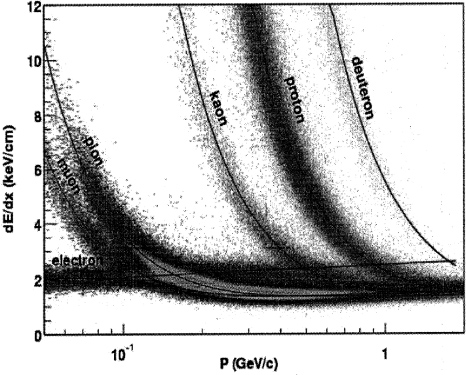
\includegraphics[width=5.5in]{../figures/0034-4885-73-11-116201_star_PID.jpg}\\
  \caption{Energy loss distribution in the STAR TPC for primary and secondary particles. \cite{0034-4885-73-11-116201}.}\label{fig:STAR_PID}
  % "Figure 35 shows the energy loss distribution for primary and secondary particles."
\end{figure}
%\Its drift volume is full of P10 gas (10% methane and 90% argon), the electrons from the molecules of which are knocked off by a charged particle travelling through the medium.

%\Spectra from the BES program (PhysRevC.96.044904 : https://arxiv.org/pdf/1701.07065.pdf)
%\ Beam Energy Scan program
%\ particle identification
%\ transverse momentum spectrum (using tracking detectors????)
%\ errors associated with the spectra

\section{The Beam Energy Scan Program}
The RHIC, in 2010, started a multi-phase Beam Energy Scan (BES) program to study the QCD phase diagram. The collider has the unique facility to collide nulclei at a range of center-of-mass energies per nucleon, $\sqrt{s_{NN}}$. It also has two different detectors that are currently operational, STAR and PHENIX (Pioneering High Energy Nuclear Interactions eXperiment), which facilitate the cross-checking of results. Between 2010 and 2011, under the exploratory phase I of the BES program, 7.7, 11.5 (not completed in PHENIX), 19.6, 27, and 39 GeV collisions were completed using pairs of Au nuclei. Together with the data formerly collected by the RHIC at higher collision energies, BES phase I data can scan the interval from 450 MeV to 20 MeV in $\mu_{B}$ space \cite{1742-6596-455-1-012037, LUO201675}. One of the things that can be studied with the data associated with this region of the phase space is statedly the possibility of a ``turn-off of new phenomena already established at higher RHIC energies" (https://drupal.star.bnl.gov/STAR/starnotes/public/sn0493). Results corresponding to the high-$\mu_{B}$ region might provide evidence of a first order phase transition, and possibly the critical point \cite{LUO201675}.

The manifestation of such phenomena would be in terms of the fluctuations in the properties of the post-collision system. One can, for instance, study the scaling of the transverse energy after the collision with the longidutional energy at the time of the collision, $\sqrt{s_{NN}}$. This can be done in multiple ways for a detector like STAR or PHENIX that is made up of sub-systems such as the TOF detectors, TPCs/Time Expansion Chambers, as well as calorimeters. 

\subsection{BES Calorimetry}
\citet{PhysRevC.93.024901} use calorimetry in PHENIX to analyze the transverse energy corresponding to several different pairs of species colliding at a range of energies. They use the raw transverse energy measured by the EMCal, $E_{{T}EMC}$, to obtain the total hadronic $E_{T}$ by making corrections in three different steps. They first scale the data by a constant factor calculated to account for the fiducial acceptance in azimuth and pseudorapidity. The second factor is calculated to adjust for the effects of the calorimeter towers that are disabled. The third factor, $k$, is computed as follows
\begin{equation}\label{eqn:AdareKfactor}
k = k_{response} \times k_{inflow} \times k_{losses}
\end{equation}
where $k_{response}$ corresponds to hadronic particles only depositing a fraction of their total energy while passing through the EMCal, $k_{inflow}$ is attributable to the energy deposited by particles coming from outside the EMCal's fiducial aperture, and $k_{losses}$ accounts for the energy not registered in the EMCal due to energy thresholds, edge effects, and more importantly due to the particles that make it into the fiducial aperture but decay into products outside the aperture.

\subsection{BES $p_{T}$ spectra}
This thesis details the method of transverse energy analysis through the use of $p_{T}$ spectra from the STAR BES data. As described in section \ref{subsec:tracking_STAR}, the TPCs and TOF detectors in STAR can identify particles as well as their trajectories and ultimately their multiplicity distributions with respect to the momenta. \citet{PhysRevC.96.044904} report the results for the $p_{T}$ spectra for six different identified hadrons, $\pi^+$, $\pi^-$, $K^+$, $K^-$, $p$, and $\bar{p}$, from the STAR experiment. The spectra come from Au+Au collisions -- at $\sqrt{s_{NN}}$ = 7.7, 11.5, and 39 GeV in the year 2010 and at $\sqrt{s_{NN}}$ = 19.6 and 27 GeV in 2011 -- under the BES Program. Figure \ref{fig:BESPaper_pTSpectra} \cite{PhysRevC.96.044904} shows the spectra corresponding to 39 GeV collisions categorized into seven different collision centralitiy classes. These spectra, and their counterparts for the rest of the energies, were used to calculate an estimate of the total transverse energy per event per particle species. This result was then used to estimate the total transverse energy due to all the collision products.
\begin{figure}[h]
  \centering
  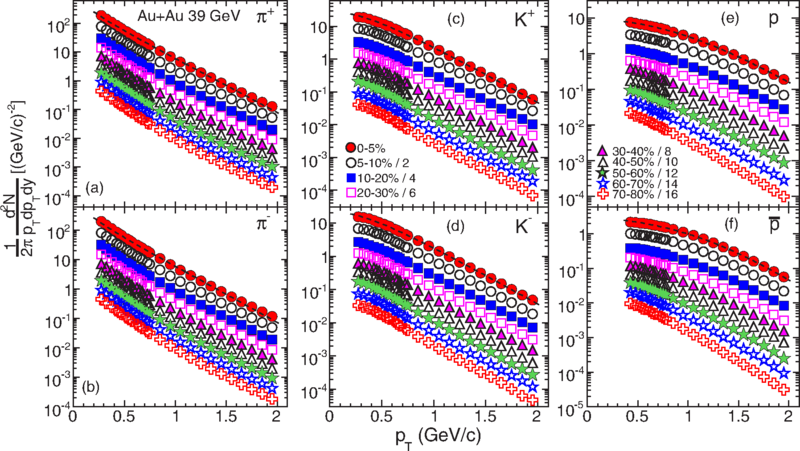
\includegraphics[width=6.5in]{../figures/PhysRevC-96-044904_pTSpectra_39.png}\\
  \caption{Transverse momentum spectra for $\pi^{+}$, $\pi^{-}$, $K^+$, $K^{-}$, $p$, and $\bar{p}$ at midrapidity ($|y|$ $<$ 0.1) from 39 GeV Au+Au collisions at RHIC. The fitting curves on the 0-5\% central collision spectra for pions, kaons, and protons/anti-protons represent, respectively, the Bose-Einstein, $m_{T}$-exponential, and double-exponential functions. \cite{PhysRevC.96.044904}.}\label{fig:BESPaper_pTSpectra}
\end{figure}

The corrections applied by \citet{PhysRevC.96.044904} to the raw data to obtain the spectra and the reported systematic uncertainties in their results are discussed below (under construction)

// Next section will contain the method of extrapolation and the section after that will explain the analysis using the root framework. Then comes the results section, which I will add after I finish analyzing all the data and get all the results including for lambdas.

%...... mathematics involved in getting ET out of pT spectra, including the extrapolation using the BGBW.............

%...... assumption leading to total ET estimate, i.e, how the scaling up is done, and the errors associated with it...............

%chapter 3: data analysis
%go through the steps from getting the data to getting the final results
%example fit plots
%justification of using chi-squared

%chapter 4: results
%plots and tables compared to what's been published.
%Anything interesting seen?

%chapter 5: conclusion
%chapter 6: future work

%acknowledgments
%christine, adam, charles, soren, andy, will, chrisanne.
%\ NEXT: WRITE ABOUT THE ALTERNATIVE WAY, THAT IS, USING SPECTRA, AND WHAT DETECTOR THIS METHOD USES INSTEAD


%\"The main detectors used to obtain the results on pT spectra, yields and particle ratios for charged hadrons are the Time Projection Chamber (TPC) [41] and Time-Of Flight detectors (TOF) [42]" https://arxiv.org/pdf/1701.07065.pdf
%\ " The TPC data is used to determine particle trajectories, thereby their momenta, and particle types through ionization energy loss (dE/dx)."
%\ "For higher momentum, we use time-of-flight information to identify particles. The TOF particle identification for this analysis is used above pT = 0.4 GeV/c."

%\Historically, measurement of $E_{T}$ would be one of the first things done after heavy-ion collisions. Electromagnetic calorimeters (EMCals) would be used to perform the measurement of $E_{T}$. 

    \chapter{Data Analysis} \label{ch:analysis}
The analysis of the data involved extrapolating the available spectra and using the results from the fits to calculate the transverse energy for all the available spectra and the particle multiplicity corresponding to charged particles. Details follow.

\subsection{STAR $p_{T}$ spectra}
This thesis details the method of transverse energy analysis through the use of $p_{T}$ spectra from the STAR BES data. As described in section \ref{subsec:tracking_STAR}, the TPCs and TOF detectors in STAR can identify particles as well as their trajectories and ultimately their multiplicity distributions with respect to the momenta. \citet{PhysRevC.96.044904} report the results for the $p_{T}$ spectra for six different identified hadrons, $\pi^+$, $\pi^-$, $K^+$, $K^-$, $p$, and $\bar{p}$, from the STAR experiment. The spectra come from Au+Au collisions -- at $\sqrt{s_{NN}}$ = 7.7, 11.5, and 39 GeV in the year 2010 and at $\sqrt{s_{NN}}$ = 19.6 and 27 GeV in 2011 -- under the BES Program. Figure \ref{fig:BESPaper_pTSpectra} \cite{PhysRevC.96.044904} shows the spectra corresponding to 39 GeV collisions categorized into seven different collision centralitiy classes. These spectra, and their counterparts for the rest of the energies, were used to calculate an estimate of the total transverse energy per event per particle species. This result was then used to estimate the total transverse energy due to all the collision products.
\begin{figure}[h]
  \centering
  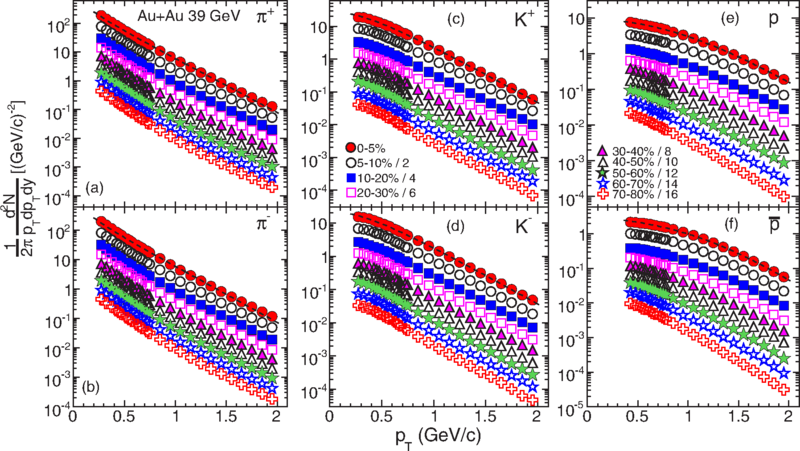
\includegraphics[width=6.5in]{../figures/PhysRevC-96-044904_pTSpectra_39.png}\\
  \caption{Transverse momentum spectra for $\pi^{+}$, $\pi^{-}$, $K^+$, $K^{-}$, $p$, and $\bar{p}$ at midrapidity ($|y|$ $<$ 0.1) from 39 GeV Au+Au collisions at RHIC. The fitting curves on the 0-5\% central collision spectra for pions, kaons, and protons/anti-protons represent, respectively, the Bose-Einstein, $m_{T}$-exponential, and double-exponential functions. \cite{PhysRevC.96.044904}.}\label{fig:BESPaper_pTSpectra}
\end{figure}

The corrections applied by \citet{PhysRevC.96.044904} to the raw data to obtain the spectra and the reported systematic uncertainties in their results are discussed below (under construction)
.....................................................................................................

\section{Extrapolation of Spectra}
The available spectra were limited to a range of transverse momenta ranging from around 0.25 GeV/c to around 2 GeV/c (for pions). To account for the transverse energy corresponding to the momenta for which there was no available data, an extrapolation had to be used. The model used for the extrapolation and the associated statistics are discussed below.

\subsection{Boltzmann-Gibbs Blast Wave}
The blast wave is a common model used in the analysis of the particle spectra.[????] The specific model used in this thesis is the Boltzmann-Gibbs blast wave (BGBW) as represented in equation \ref{eqn:bgbw}. It has the parameters mass, temperature, beta, v, and n. I assume that any anomalies in the magnitude of the normalization parameter do not affect the results significantly insomuch as they don't lead to: 

(a) unreasonable relative errors in the extrapolated values of the transverse energy,

(b) any of the spectral fits having the extrapolated transverse energy more than that calculated from just the available spectra, and

(c) for the 200 GeV collision samples, at least, the extrapolation at higher $p_{T}$ being more than that at lower $p_{T}$.

	\begin{equation}\label{eqn:BGBW}
	BGBW
	\end{equation}

\subsection{Fitting Spectra to BGBW}
Figure \ref{fig:fit} presents an example of a Boltzmann-Gibbs Blast Wave (BGBW) fit on one of the individual particle spectra with the goodness-of-fit as well as other statistics and the associated errors. A parallel-coordinates plot is presented in the next chapter in fig. \ref{fig:parallelCoord}, which shows the measured centralities, two of the good-fit parameters, and the calculated transverse energies for 270 different particles (lambdas not included).

	\begin{figure}[h]
	  \centering
	  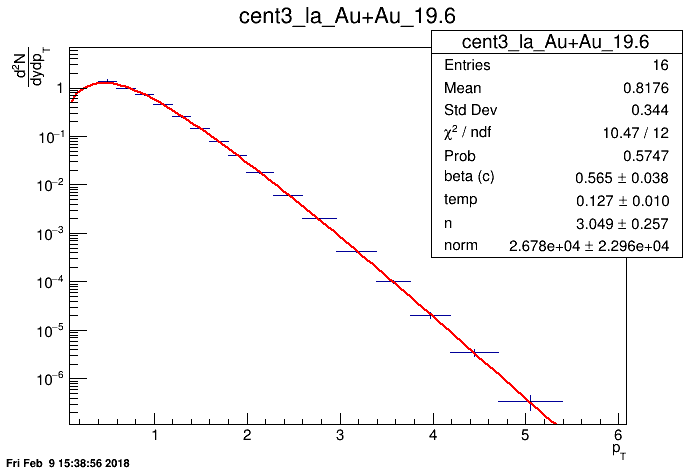
\includegraphics[width=4.5in]{figures/cent3_la_Au+Au_196.png}
	  \caption{Red curve shows the Boltzmann-Gibbs blast wave functional fit on the PRELIMINARY transverse momentum spectrum for lambda particles identified by the STAR detector for 19.6 GeV Au+Au collisions (10-15\% central). Parameters extracted from the chi-square goodness-of-fit test, as well as other statistics, are shown in the box on the top right.}\label{fig:fit}
	\end{figure}

\section{Calculations from the Spectral Fits}
\subsection{Calculation of $\frac{dE_{T}}{dy}$, $\frac{dE_{T}}{d\eta}$, $\frac{dN_{ch}}{dy}$, and $\frac{dN_{ch}}{d\eta}$}
\subsection{Corrections for Unidentified Particles and Estimation of Total $E_{T}$}
It is reasonable to assume that, at high energies, there should be roughly the same multiplicity of all the isospin states of a final state particle. Table \ref{table:isospinStates} lists the isospin states associated with the pion, the kaon, the proton, and the lambda particles.

	\begin{table}[h!]
	\centering
	\begin{tabular}{|c c|}
	%\tabletypesize{\scriptsize}
	%\rotate
	\hline
	Particle & Isospin multiplets \\ [0.5ex]
	\hline
	\hline
	pion & $\pi^{+}, \pi^{0}, \pi^{-} $ \\
	kaon & $K^{+}, K^{0}, K^{-}, \bar{K}^{0}$ \\
	proton & $p, n$  \\
	lambda & $\Lambda$  \\ [1ex]
	\hline
	\end{tabular}
	\caption{Isospin states of different identified particles.}
	\label{table:isospinStates}
	\end{table}
	
	.............text content.............
	
	\begin{equation}\label{eqn:TotET}
	E_{T} = 3E_{T}^{\pi} + 4E_{T}^{K} + 4E_{T}^{p} + 2E_{T}^{\Lambda}
	\end{equation}
	
 ................text content...................
 
\subsection{Lambdas Centralitiy Adjustments and $E_{T}$ Interpolations}
The centrality bins corresponding to the lambdas spectra were slightly different from those corresponding to the rest of the particles........
%\subsection{}
\section{Uncertainties}
......... 100\% correlated point-to-point and uncorrelated between particles........ ?
%\section{}

    \chapter{Summary and Conclusions} \label{ch:conclusions}

The purpose of the measurement described in this work is to address issues concerning cold nuclear matter effects in the production of the heavy flavor quarks in relativistic heavy ion collisions. Is the yield of heavy flavor produced in collisions affected by the additional nucleons present in proton-nucleus collisions as compared to proton-proton collisions? Additionally, is the production and momentum distribution of heavy quarks affected differently from light quarks? Furthermore, are there new physics effects at the high LHC energies as compared to what has been previously measured at RHIC?

In order to address these questions, the Large Hadron Collider accelerated and collided protons at 4 TeV with lead ions at 82x4 TeV. These asymmetrical proton-lead collisions at center of mass energy per nucleon $\sqrt{s_{NN}} = 5.02$ TeV were measured by ALICE. This analysis measured the yield of mesons composed of one charm or bottom quark and a light quark, $D^+ , D^- , D^0 , \bar D^0, B^+ , B^- , B^0 , \bar B^0$. The production of $D$ and $B$ hadrons were measured through their semileptonic decay channel by measuring the single electron yield. 

Electrons were enhanced by using the tracking and energy measurements provided by the Time Projection Chamber and the Electromagnetic Calorimeter. The remaining hadron contamination was subtracted with a function that was fit to the detector response of the electron signal and the hadron background. This measurement covered a novel transverse momentum range made possible by the EMCal trigger system. However, these triggers introduced an additional background that needed to be accounted for in the background subtraction. 

The main sources of background electrons are from photon conversion and from Dalitz decay of light mesons. This analysis estimated the yield of background electrons by exploiting the fact that the main background sources produced electrons in pairs with an invariant mass near zero, while the signal produced single electrons. 

The final results of the yield, cross section, and $R_{pPb}$ of electrons from the decays of $D$ and $B$ mesons in $pPb$ collisions as measured in ALICE at the LHC were presented in figure \ref{fig:HFEYieldAllTriggers}, figure \ref{fig:HFECSCombined} and figure \ref{fig:CombinedRAAFONLL}.

This analysis extended the transverse momentum reach of an earlier measurement in ALICE \cite{Adam:2015qda}. The measurement of the cross section agrees with the earlier measurement as shown in figure \ref{fig:PubAndRebCSCombined}. The transverse momentum coverage of this analysis was able to extend the $p_{T}$ reach of the previous measurement from 12 GeV/c up to 30 GeV/c using the EMCal triggers. 

The $R_{pPb}$ of this measurement demonstrated agreement with the previous measurement in the $p_{T}$ overlap region in figure \ref{fig:RebeccaAndJanRAA}. A similar analysis, that reconstructs the D meson using the hadronic decay channel, was also shown to agree with the measurement from this analysis in figure \ref{fig:Dmesons}.

Theoretically the data are well described by FONLL, Fixed Order plus Next-to-Leading-Log perturbative Quantum Chromodynamics theory calculation with standard parameters. The pQCD theory was calculated for proton-proton collisions and then scaled using the average number of binary nucleon-nucleon collisions to compare with proton-lead collisions illustrated in figure \ref{fig:CombinedCSandScaledFONLL}. FONLL describes the data well across six orders of magnitude. More advanced models that take into account various cold nuclear matter effects were also consistent with this measurement, as depicted in figure \ref{fig:RebeccaAndJanRAA}.

This measurement was compared a similar collision system, $d+Au$, at a lower energy, $\sqrt{s_{NN}} = 200$ GeV measured at RHIC. Figure \ref{fig:DAuPhenixAndMineCombined} shows a slight possible Cronin enhancement at low $p_{T}$ and is consistent with unity at higher $p_{T}$. These results show that the effects of cold nuclear matter in $pPb$ collisions as compared to $pp$ collisions are small for heavy flavor hadrons at LHC energies and do not deviate significantly from the measurements at RHIC energies.

As seen in figure \ref{fig:PionsKaonsProtons}, the $D$ and $B$ mesons seem to scale similarly to other light flavored charged hadrons when comparing $pp$ to $pPb$ collisions. The modification of light and heavy quarks are comparable in $pPb$ collisions.

Figure \ref{fig:DAuPhenixAndMineCombined} and figure \ref{fig:2016-Sep-23-hfe_00_10RHIC} illustrate a significant suppression in heavy ion collisions, $Au+Au$ and the $Pb-Pb$, at RHIC and LHC energies. Since the $d+Au$ and $pPb$ collision data does not show any signs of suppression on heavy flavor, initial state effects and cold nuclear matter effects can not explain the suppression seen in central heavy ion collisions and must be due to hot nuclear matter effects.







    %%%%%%%%%%%%%%%%%%%%%%%%%%%%%%%%%%%%%%%%%%%%%%%%%%%%%%%%%%%%%%%%%%%%%%%%%%%%%%%%%%%%%%%%%%%%%%%%%%%%%
    % BIBLIOGRAPHY
    %%%%%%%%%%%%%%%%%%%%%%%%%%%%%%%%%%%%%%%%%%%%%%%%%%%%%%%%%%%%%%%%%%%%%%%%%%%%%%%%%%%%%%%%%%%%%%%%%%%%%
    \renewcommand{\bibname}{}
    \makeBibliographyPage  % make the bibliography title page - can be edited in ut-thesis-template.tex
    \bibliographystyle{unsrt}%was plain, apalike, unsrt  bibliography style - recommend using apalike-doi as it hyperlinks DOIs
    \hypersetup{urlcolor=black}
    \bibliography{references/references-Rebecca} % references.bib included in the references directory
    %%%%%%%%%%%%%%%%%%%%%%%%%%%%%%%%%%%%%%%%%%%%%%%%%%%%%%%%%%%%%%%%%%%%%%%%%%%%%%%%%%%%%%%%%%%%%%%%%%%%%
    % APPENDIX - OPTIONAL - COMMENT IF NOT NEEDED
    %%%%%%%%%%%%%%%%%%%%%%%%%%%%%%%%%%%%%%%%%%%%%%%%%%%%%%%%%%%%%%%%%%%%%%%%%%%%%%%%%%%%%%%%%%%%%%%%%%%%%
%    \addToTOC{Appendix}
%    \makeAppendixPage   % make the appendix title page - can be edited in ut-thesis-template.tex
%    \appendix
%    \chapter{Summary of Equations}
\section{Equations}
some equations here

    %%%%%%%%%%%%%%%%%%%%%%%%%%%%%%%%%%%%%%%%%%%%%%%%%%%%%%%%%%%%%%%%%%%%%%%%%%%%%%%%%%%%%%%%%%%%%%%%%%%%%
    % A VITA IS REQUIRED
    %%%%%%%%%%%%%%%%%%%%%%%%%%%%%%%%%%%%%%%%%%%%%%%%%%%%%%%%%%%%%%%%%%%%%%%%%%%%%%%%%%%%%%%%%%%%%%%%%%%%%
    \addToTOC{Vita}
    \chapter*{Vita} \label{ch:vita}
Vita goes here. The vita should be a brief biography about the author written in third person and paragraph format. It should not be the author's resume or CV.
\end{document}
